\chapter{Implementation}

In this chapter we will take a close look into the overall functioning of an football articles generating NLG system. The goal was to create an end-to-end NLG system, that takes non-processed raw data about a football match as an input and creates article in Czech language that summarises the development of a match. The aim of the thesis was not only to get the basic understanding of a NLG process, but also try to create the implementation in a language that is widely used around the world and for me, personally, was less known - Python.

\section{Requirements and initial goal}
As mentioned in the introduction of this section, the expected output was simply a readable Czech text summary while attempting to produce sentences that are not identical resulting in less-monotonic text. Since the expected output was defined as somewhat vague and quality-wise uncertain, there is no stress on the definition of goal of the language and target audience. However, the text quality, especially in the variability of expressions, used structures and overall richness, is insufficient to truly satisfy the definition of an article. 

Since NLG is a complex process we used one already existing tool for linguistic realisation - \emph{Geneea API}. Without this tool the output language would not be grammatically correct and therefore not satisfying the readability requirement. As discussed in (TODO-A-ref na linguistic realisation) this task has no easy way of implementing manually, especially not for a Czech language that belongs to the most complicated natural languages (for reasons that are described in (TODO-A-ref na linguistic realisation)). \emph{Geneea API} usage skips this task focusing on the rest of the NLG tasks combined.

In \autoref{chap:process} (TODO - A - ref a whole section) We proposed an outline to a requirements analysis. This section will follow this structure describing the specifics.

\section{Input data}
Dataset was provided by a company Livesport s.r.o. (TODO-A-mám ji zmiňovat), which I would like to thank. Therefore entire dataset can not be shared. However, one example match is attached to illustrate program functioning. Initial dataset is composed of every match of one Czech First League season. Every match is represented as JSON file storing both general information about the match (teams, venue, attendance, line-ups, etc.) and course of key events of the matches (goals, substitutions, cards, etc.). 

General information about the match consists of two participating teams, starting time of the match, tournament information (here it is Czech First League for the particular year), information about venue, score, winner, stage of the game (e.g. finished/delayed) and line-up. Line-up consists of every player of the team divided into groups according to their status (e.g. injured, benched, initial line-up, etc.) among with other information like home country, number and more. 

Course of events is represented as a list of incidents. Incident has attributes like id, time, participant, type and so on. Also, incidents have attribute \emph{parentId}, which further specifies the incident. For instance incident type \emph{Penalty Kick} has empty \emph{parentId}, however, in incidents there is incident type \emph{Penalty Scored} or \emph{Penalty Missed} that has \emph{parentId} identical to corresponding \emph{Penalty Kick} \emph{Id}. 

\section{Approach}

For this NLG problem I have chosen modular architecture as described in (TODO-A-ref section) - the most traditional, even though now a little outdated, approach proposed by \cite {reiter1997building} consisting of grouping similar NLG tasks into modules that are then connected via one-way-pipeline. 

In the first place, I would like to highlight the reasons that led to a chosen approach:
\begin{itemize}
	\item My personal lack of experience in NLG as this was my first ever NLG system that I have created.
	\item The lack of easily accessible big amount of data.
	\item The full extent of a NLG problem - from non-processed data to well-built text.   
\end{itemize}

For me, personally, this field of computational linguistic is new and therefore the aim  was not only to build a NLG system, but gain knowledge including different approaches in this specific subfield of NLP. Staying faithful to the division of modules is the most intuitive and also feasible solution, which closely relate to the point of the end-to-end extent of the problem. It was easy for me to get lost in the high amount of issues to resolve (each of the NLG tasks) without giving it a properly divided structure. Also the error propagation was another problem that has risen from the lack of experience.

In addition, the lack of data almost forbids the data-driven approach. Naturally, the data do exist, but their acquisition would require either high amount of time consuming labour of creating the data by hand or developing football articles automatically and then aligning them with given input data, which still can end up insufficient as for the acquired text more data could have been known. Such a corpus building could be a project on its own.

\section{Match example}
A match example is provided and the summary can be seen in \figref{overview}. 

Football match between \emph{Jablonec} and \emph{Bohemians 1905}, which resulted in a 3 to 1 victory for the home team \emph{Jablonec}. First half can be summarised in words to further describe the figure: First goal was a penalty scored by \emph{Trávník} in 10th minute and then second incident was a goal by \emph{Bohemians'} player \emph{Hašek} that tied the game in 44th minute after a pass from \emph{Vaníček}. Events that happened in second half are hopefully easy to interpret as well. Numbers next to a incident group them by their type- (1) penalty goal, (2) goal with an assist, (3) substitution and (4) yellow card. 

\begin{figure}[p]
	\centering{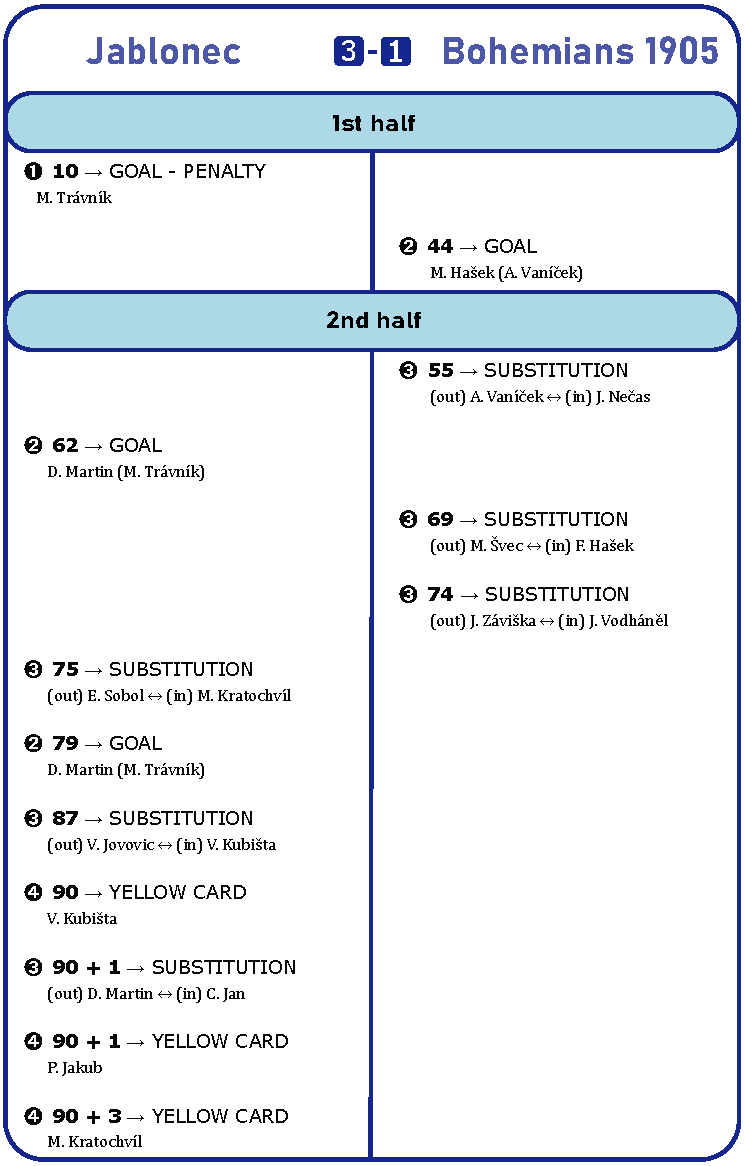
\includegraphics[width=0.9\textwidth]{../img/match_overview.pdf}}
	\caption{Table summary of the example match.}
	\label{fig:overview}
\end{figure}

\section{Structure overview}
The overview of the structure of the solution is shown in \figref{structure}.

Input data with arguments to modify slight functioning (as way of output, or number of texts to generate) are passed to \emph{run.py} (\figref{structure} - 1) (.py will be left out as it is implicit for every module), which is the executable starting point of the program. Parsed arguments are an input for \emph{articles\_generator}, which handles the communication between each module, essentially creating the one-way-pipeline for modules (\figref{structure} - 2, 3, 4, 5) and managing passing the suitable inputs and outputs. Output of this core handler is tuple of strings - title and body of the article.

The \emph{data\_initializer} (\figref{structure} - 2) is as module not present in the original module architecture by \cite{reiter1997building} (described in (TODO-A-odkaz na sekci)). However, since the data is in a raw form, the step of data processing needed to be added to store the data in a more convenient way to further operate with the information given.

Modules (\figref{structure} - 3, 4, 5) correspond to the modular architecture perfectly. \emph{Document\_planner} (\figref{structure}-3) takes data about a match in a convenient inner representation. Creating a \emph{DocumentPlan}, which contains preverbal messages to be said in a sentence. Then these messages are lexicalized in \emph{sentence\_planner} (\figref{structure} - 4) and finally linguistically realised by \emph{linguistic\_realiser} (\figref{structure} - 5). 

Moreover, there are three auxiliary modules to keep the structure of the implementation as clean as possible:
\begin{itemize}
	\item \emph{Data.py}
	\item \emph{Types.py}
	\item \emph{printer.py}
\end{itemize}
These are further described later in (TODO-ref).

\begin{figure}[p]
	\centering{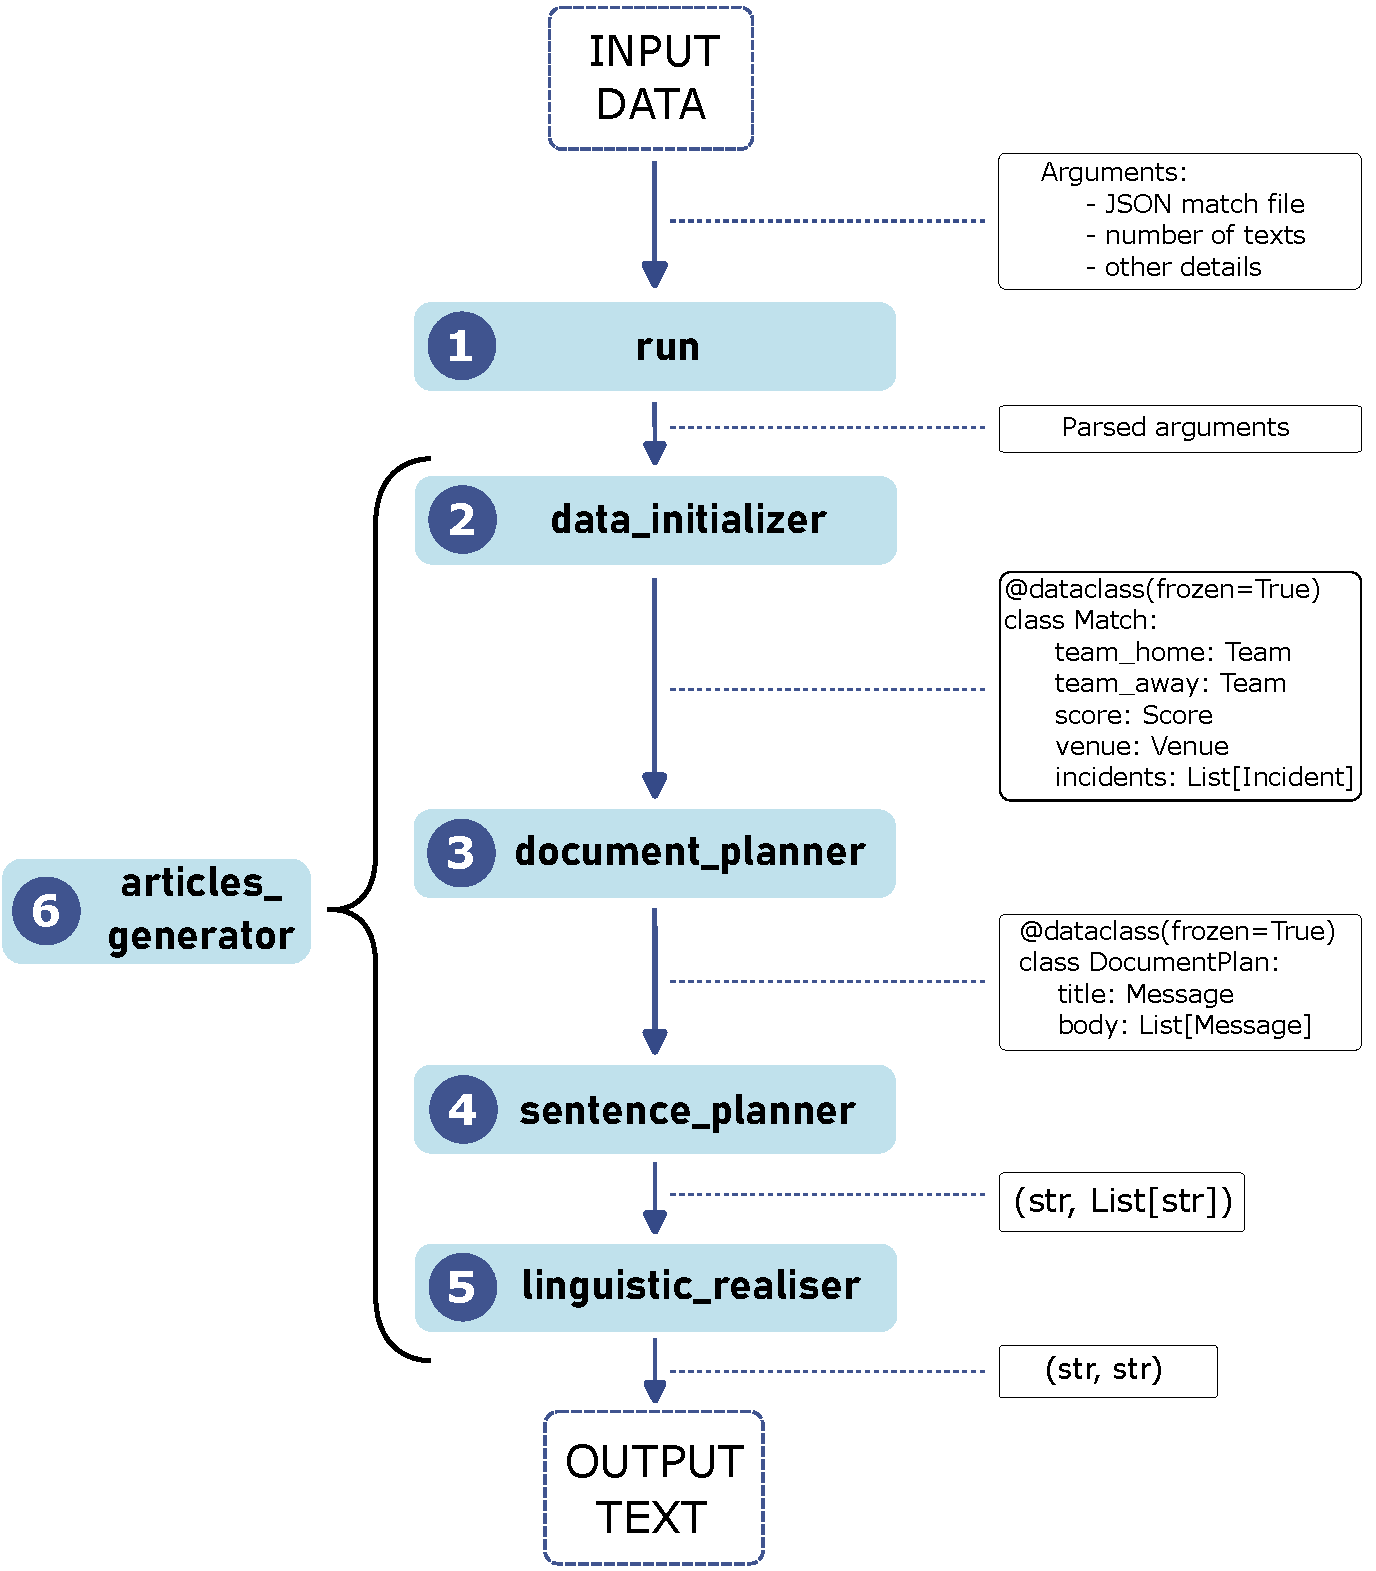
\includegraphics[width=1\textwidth]{../img/program_structure.pdf}}
	\caption{Overview of solution structure.}
	\label{fig:structure}
\end{figure}

\section{Modules implementation}
In this section the implementation of each module is described in detail creating a compact solution in Python. I

\subsection{Auxiliary modules}
\textbf{\textit{Data.py}} groups data classes that store information contained in a JSON file. Namely these entities are \emph{Score, Venue, Country, Player, Team, Time, Incident (+IncidentParent) } and finally the most crucial \emph{Match} that encapsulates each of the class mentioned. Note that these classes are made immutable using \emph{@dataclass(frozen=True)} from package \emph{dataclasses} and then implementing static \emph{create} method. Immutability ensures the data remain intact after manipulating with them frequently in multiple functions across modules. 

Module \textbf{\textit{printer.py}} manages printing different components in a readable way. Since there is a lot of data, even during the development it was more convenient to pretty-print separate results of modules instead of inspecting more nested and complicated states during debugging. Due to numerous alignments and length of string appending separate module was created to not overload other segments of the code.

Lastly, \textbf{\textit{Types.py}} stores enumarate types for different entities. For instance, in module \emph{document\_planner} there is a class \emph{Message} to store attributes of a preverbal message. One of the attribute is type of the message defined as \emph{Types.Message}. This class is implemented in \emph{Types.py} (along with other types, which have arisen so often that separate module was created) as Python's \emph{enumerate()}. Options are \emph{GOAL, PENALTY\_KICK\_MISSED, CARD, SUBSTITUTION, RESULT}. To give one more example, message that reports a card has attribute about type of card stored in \emph{Types.Card} - \emph{YELLOW, RED\_AUTO, RED\_INSTANT} (distinguishing the difference between two yellow cards and instant red card - to highlight the severeness of the foul). Similarly, other types of different-level entities are stored. 

\subsection{Data initializer}
Goal of \textbf{\textit{Data\_initializer}} is to transform data from initial JSON file to more convenient inner representation implemented as system of classes to uphold the principles of object-oriented programming resulting in crisp and well-divided structure.

The implementation is straightforward - we use built-in package \emph{json} to ease the manipulation with a JSON file while initializing classes from module \textbf{\textit{Data}}. 

Two examples of specific records contained in JSON file and their Python representation are shown in \figref{player} and \figref{incident}. 

\begin{figure}[h]
	\centering{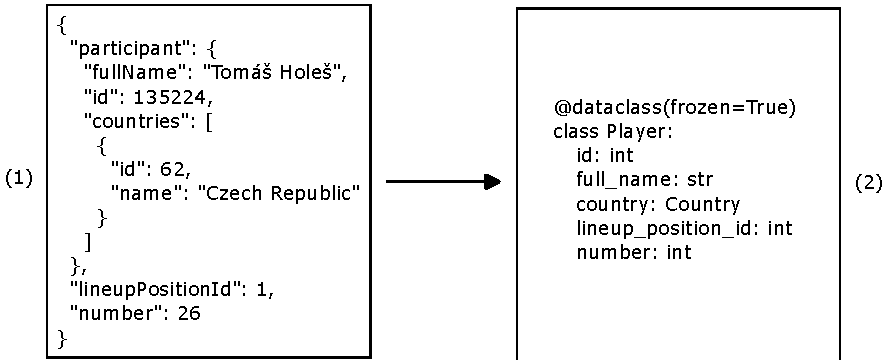
\includegraphics[width=0.9\textwidth]{../img/data_player.pdf}}
	\caption{Transformation of entity \emph{Player} from JSON to a Python class.}
	\label{fig:player}
\end{figure}

Entity {Player} is transformed from its initial JSON representation (\figref{player} - 1) to a easy-to-work-with Python's immutable class \emph{Player} with corresponding attributes. Note that a country has also a proper class \emph{Data.Country}.

\begin{figure}[h]
	\centering{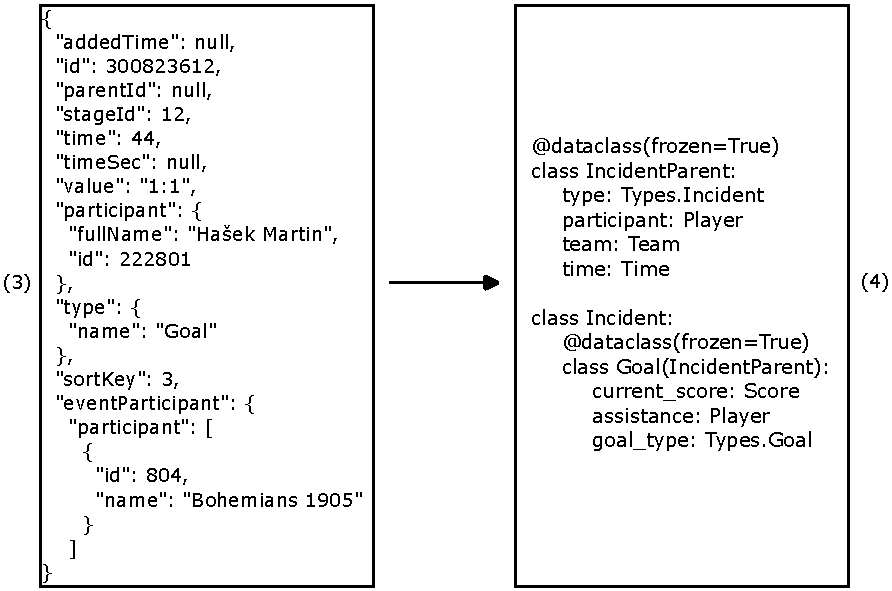
\includegraphics[width=1\textwidth]{../img/data_incident.pdf}}
	\caption{Transformation of entity \emph{Incident} from JSON to a Python class.}
	\label{fig:incident}
\end{figure} 

Entity \emph{Incident} is transformed from JSON (\figref{player} - 3) to a representation as an immutable Python's class (\figref{player} - 4). The class is called \emph{Goal} and it is a subclass of \emph{Incident}. This particular class structure ensures class addressing different types of incidents (goal/card/substitution/penalty kick) as one variable type and therefore enabling the \textit{Data.Match} class to have attribute \textit{incident} storing incidents as \emph{List[Incident]}. Furthermore, every \textit{Incident} subclass also inherits from \emph{IncidentParent} class since these are common attributes for every match incident and it would be inefficient to repeat those attributes multiple times.

Note that this module resolves part of content determination since number of attributes from initial JSON file are not transformed into Python class. For instance starting time of the match was not saved since I personally mark this information as redundant for a article generating. Similarly, more attributes were omitted to avoid useless information. On the other hand, couple attributes end up redundant (e.g. \textit{Country} of \textit{Player}), but these attributes are kept to ensure integrity of the solution and enabling easier further future development. 

\subsection{Document planner}

The aim of this module is to plan the content of the separate messages and their order. Document planner is resolved trivially - each incident is transformed to a separate preverbal message along with fundamental data. 

Implementation is shown in \figref{message} and is similar to Incident structure. Each preverbal message has different arguments and therefore own class. To access messages classes as one variable type there is a system of inheritance, where every message class inherits from \textit{MessageParent} so that they can be distinguished by their according type \textit{Types.Message}. Note that these classes again immutable to ensure data stability.

Unlike message class \textit{Substitution}, which is self-explanatory, classes \textit{Result} and \textit{MissedPenalty} need clarification. 

\textit{Result} message defines the title of the article. The core purpose of the title is to summarise a match in one sentence and hence to report the result/score of the match. 

Content of the \textit{MissedPenalty} is rather obvious, but the reasoning behind the existence of this separate class may not be visible at first glance and relies heavily on domain knowledge. Penalty is a crucial, rare and thrilling event during a football match.\footnote{Remember the famous penalty by Antonín Panenka in European Championship finals in 1976 that led to triumph of Czechoslovakia. The kick was groundbreaking and nowadays term 'Panenka' refers to a style of kick, where you only chip the ball in the middle of the net.} Consequently, every penalty is worth mentioning regardless of the outcome. However, if the penalty is successful the outcome is a goal and we would like to treat the message the same as any other goal. I believe every goal in a football match should be reported since scoring in football is rarer than in other sports in general (compared e.g. to basketball where reporting every basket would be too specific and unnecessary). Contrastingly, the message that reports a missed penalty is not required to be present in the article as this event did not affect the result directly and creates rather a shocking element of the article as players are expected to score from this position. This paragraph further illustrates the hand-crafted principles based on the domain knowledge that are incorporated in the solution.

\begin{figure}[h]
	\centering{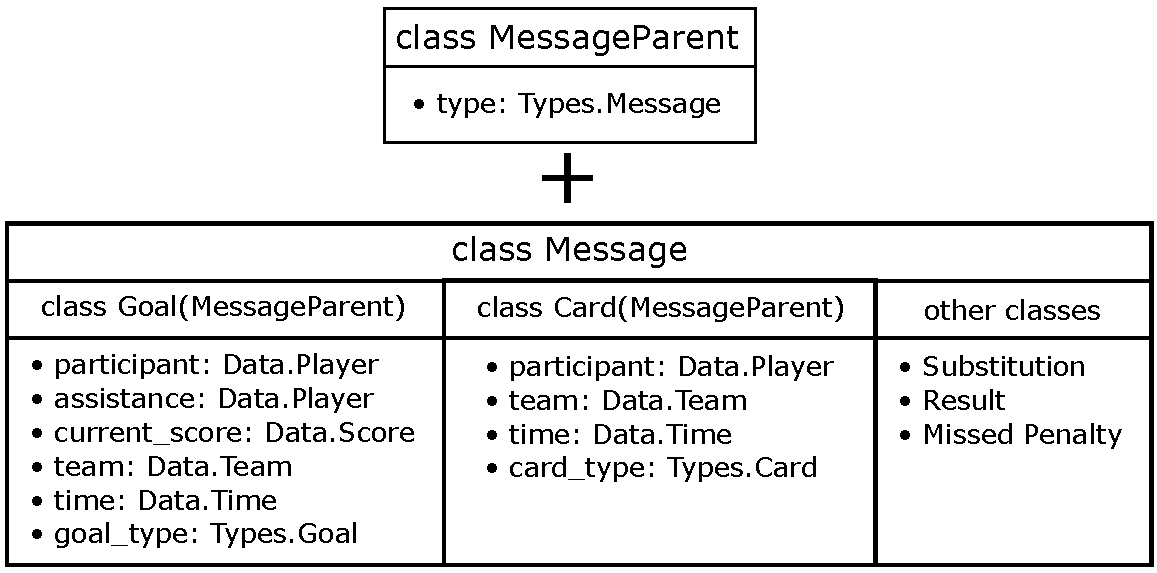
\includegraphics[width=1\textwidth]{../img/message_implementation.pdf}}
	\caption{Implementation of preverbal messages.}
	\label{fig:message}
\end{figure} 

\subsection{Sentence planner}
Last but not least is a sentence planner, that combines sentence aggregation, lexicalization and REG. Due to possible low number of messages to convey depends heavily on the course of the game, sentence aggregation is not performed. To further simplify process one incident corresponds to one sentence.

The core idea is to exploit method of templates, which is inserting words to express constituent (e.g. entities to be expressed from non-verbal message) verbally in the reserved empty spot in the sentence. However, to ensure some kind of variability as well as easy cooperating with Genja API the templates are resolved in a bit more complex way. Naming classes and variables throughout sentence planner was difficult due to the similarities of the segments that needed to be named, therefore I first present crucial classes and reveal their principle.

Firstly, the template, by its very nature, is represented as a class called \textit{\textbf{Sentence}}. \textit{Sentence} controls the structure of the sentence and allow other components of the implementation to insert various lexical items. \textit{Sentence} contains string \textit{id} to simplify number of types and subtypes in this section. Boolean \textit{simple} says whether the expression is simple, clear, syntactically easy or the opposite: colourful, longer and more complex. Then there is list of \textit{constituents}, which is either a hand-inserted string or \textit{Constituent}, that requires further development and will be picked later. Note that \textit{Sentence} consists attribute \textit{msg}, but the attribute is not assigned immediately.
\begin{Verbatim}[frame=single]
class Sentence:
	id: str
	simple: bool
	constituents: List[Union[str, Constituent]]
	msg: dp.Message
\end{Verbatim}
Here is an example of one \textit{Sentence} initialization, which defines the easiest possibility how to express a message that a goal was scored. Furthermore, following table shows possible lexicalization of these constituents in English(EN) and Czech(CZ) to illustrate the principle of such a structure.\footnote{Note that the order of the words is not correct in English, but correct in Czech. My translation will mainly illustrate the process for English readers, which can lead to grammatically incorrect sentences or expressions.}

\begin{Verbatim}[frame=single]
Sentence.create(type_, subtype, True, [
  Constituent(id_='e-time', morph_params='',
  	explicit_data=Types.ExplicitEntityData.TIME),
  Constituent(id_='v-goal', morph_params='.-0-.-.-.',
  	explicit_data=None),
  Constituent(id_='e-player', morph_params='1-.-0-.-.',
  	explicit_data=Types.ExplicitEntityData.PARTICIPANT),
  Constituent(id_='w-goal', morph_params='4-.-.-.-.',
  	explicit_data=None)]))
\end{Verbatim}

\begin{center}
	\begin{tabular}{ |c|c|c|c|c| }
		\hline
		 & Time & Verb for goal &Player entity &Word for goal \\ \hline
		 & e-time & v-goal & e-player & w-goal \\ \hline
		EN &In 7th minute& scored & Ronaldo & goal. \\  
		CZ & V 7. minutě & dal & Ronaldo & gól.\\
		\hline
	\end{tabular}
\end{center}

Another class is \textit{\textbf{Constituent}} containing again \textit{id} to mark its type or subtype. In Czech multiple agreements as well as grammatical cases need to be resolved and therefore we have to store such information when creating sentence layout regardless of the lexical expression that will be inserted. All morphology attributes are stored in \textit{morph\_params} containing case, tense, gender and ref/agr all to be then handed over to Genja API for linguistic realisation. Again, as seen in the \textit{Sentence} initialization, \textit{morph\_params} are initialized using string \textit{id}.

\begin{Verbatim}[frame=single]
class Constituent:
	id: str
	morph_params: MorphParams
	explicit_data: Types.ExplicitEntityData   
	string: str   
\end{Verbatim}

Lastly, class \textit{\textbf{Template}} handles the last step: how to lexicalize a constituent. 
\begin{Verbatim}[frame=single]
class Template:
	id: str
	string: str
\end{Verbatim}
\textit{Templates} can be strings, or a part of entity information can be inserted into a lexical item. \textit{Template}'s string can be defined by hand, or by function or by creating a template (by combining string and variables), which expresses the constituent. Here are examples for templates that express player entity and a word for assistance.

\begin{center}
	\begin{tabular}{ |c|c|c| }
		\hline
		\multicolumn{3}{| c |}{Entity player (e-player)} \\ \hline
		String for template & EN & CZ \\ \hline
		player.full\_name & Cristiano Ronaldo  & Cristiano Ronaldo \\
		player.get\_last\_name() & Ronaldo & Ronaldo \\
		"hráč číslo \$player.number" & player number 7 & hráč číslo 7 \\
		\hline
	\end{tabular}
\end{center}

\begin{center}
	\begin{tabular}{ |c|c| }
		\hline
		\multicolumn{2}{| c |}{Word assistance (w-assistance)} \\ \hline
		 EN & CZ \\ \hline
		assistance  & asistence\\
		pass & přihrávka \\
		\hline
	\end{tabular}
\end{center}

To recapitulate, class \textit{Sentence} creates templates for sentence combining and ordering numerous constituens, which are either hand-written string or represented as internal \textit{Constituent} class. For every \textit{Constituent} an instance of the class \textit{Template} is created to then present options for expressing \textit{Constituent} numerous ways.

To manage these objects and enable their cooperating, two handlers are created: \textit{SentenceHandler} and \textit{TemplateHandler}. \textit{Sentences} are first initialized all, then randomly shuffled and lastly grouped by their id and always using simple sentence first. Then for each message in the article a \textit{Sentence} is picked in the order they were grouped and message is assigned to the \textit{Sentence} as attribute \textit{msg}. Once every \textit{Sentence} for given message type is used, we pick randomly from used. This process ensures structural variability as we use same \textit{Sentence} twice only in case that we used all of the \textit{Sentences} for a given message.

To further increase variability of the created sentences similar process is repeated for \textit{Templates}. \textit{Templates} are randomly picked from non-used options. Once every template is present in the output, we pick random from every template ensuring we do not use same template twice in a row.

\subsection{Linguistic realiser}
Czech language is quite a complex language and therefore resolving the problem of realising chosen lexical items correctly by-hand without a proper tool performing complex morphology transformations is not efficient. This is the last step of the entire NLG, however, without the realisation the outputted text will not be readable. Therefore other software was used in order to perform linguistic realiser.

The system is called Genja provided by Geneea. Genja system, which was based on Jinja, operates with smart templates. In order to work with templates efficiently, Genja offer tools for managing morphology and knowledge base. Note that authorization key is required in order to perform linguistic realisation. This key stored as system environment variable to not be visible in a public GitHub repository. I would once more like to thank my supervisor for this possibility.

Due to the strict syntax that need to be inputed in a Genja API request, number of transformations need to be done. Firstly, combining plain string in a template with morphological parameters creating a well-built input for Genja. Secondly, json file for Genja must be created and lastly the output must be transformed from json back to string.

\subsection{Articles generator}
To finalize, articles generator connects modules together creating a notional one-way pipeline. 

\section{Output}
Since the lexical items are picked randomly, the output can contain sentences that are suboptimal and hard-to-read. For example when describing substitution message, realisation of two player entities can result in unappealing text, where it is not clearly visible who is the first and second player:
\begin{center}
	\textit{V 74. minutě střídal Vodháněl Kratochvíla Miloše.(CZ)}
	\textit{In 74th minute subbed Vodháněl Kratochvíla Miloše.(EN)}
\end{center}
Moreover, due to the international nature of football domain, often finding grammatically correct form of foreign name is not easy and Genja can not resolve this issue. 

To compensate these minor problems we output multiple texts instead of just one. As said, randomness can highly effect the overall impression from the text. When generating multiple texts the probability that one output will feel better than others is then increased. The idea of generating more than one text and then picking the best result of all generated can be useful, when the quality of the outputted text can not be ensured. However, the process of picking "the best" result can be again approached differently. For instance, using a human evaluation. Another option is to exploit the data-driven methods and pick the version that is statistically the most similar to the texts in acquired set of e.g. football articles from websites. The problem of selecting "the best" option is not solved in this project. 

Here is an example of lexicalization and realisation of one preverbal message:


As you can see the template system used created a variety of sentences.


Celé zápasy:

\section{Discussion}
In this section we discuss numerous perspectives and aspects of the solution.

First to discuss is the choice of the approach. The implementation strictly follows the division described in modular approach exploiting the power of splitting the extremely complex NLG problem into smaller easier-to-manage segments. As discussed earlier, the raw power of data can contribute to the quality of the result and therefore the first improvement of the project would be to change approach completely supposed you acquire the corpus data. However, stochastic approach rely on big amount of quality data, which are not available for me or rather their requirement would be insanely time-consuming. Moreover, this was my personally first NLG project. Due to my inexperience and lack of large number of easily accessible data the modular approach was chosen.

Naturally, quality of football articles created by sport journalists can hardly be matched with quality of outputs from the FootballArticlesGenerator software. The aim of the outputs were to be readable and form a proper Czech sentence filled with information about a football match, which was achieved. What is more, an increased variability was achieved to make text more fluid.

The complexity of the implementation was hard to deal with and not seeing the error propagation consequences the attempts of creating fully functioning system often failed. Retrospectively, the incorporated system of "two-layered" templates (implemented as \textit{Sentence} and \textit{Template}, which both fit to the template idea) is not-optimal. As seen in initializing \textit{Templates} for \textit{Time}. Firstly, the templates are picked randomly without context, meaning we can use expressions like "Two minutes after that" and so on. Secondly, to express time more variably we would like to use another template layer connected to a set of morphological parameters to be passed to Genja, but that is not possible. The best improvement for this project would be to re-implement sentence planner and using tree structure of templates to enable having template in a template. 

Such a tree structure would then require some non-trivial design and implementation to deliver the expected result. Sentences represented as trees where nodes are either strings or templates should be pre-created  to ensure variability between the sentences used throughout the text. Then the sentence aggregation can be performed once the content of the sentences is known. Lastly, lexicalizing each template in the sentence tree by various expressions. The core problem when designing this system is interconnection between the tasks, that requires a decent amount of flexibility of the tree structure in terms of implementation.  

Consequence of the well-implemented tree structure would be a better quality article. Due to the kept approach of using templates, the level of the result would not still be near to texts produced by humans. Templates offer only a number of varieties in comparison to a complex human language. Naturally, the higher the number of templates the more variable the text will be, initially approaching the human-like level. 

In addition, the database used for this project does not contain enough information to create somewhat complex article. Primary insufficiency is in the lack of details of incidents contained in the data. Expressing a goal is usually accompanied by a slight description of how the goal was scored: cross from the left side and top corner header, chaos in front of the net resulted in a rebound and a goal, beautiful solo play, 30 meter absolute screamer, etc. Similarly, the minor incidents like corners, shots, fouls, offsides are not present and could help when conveying more detailed text describing the true course of the game and not only major incidents. Lastly, there are no statistics and knowledge base present. When lexicalizing Cristiano Ronaldo we have only options to use number or name, while journalist would use more complicated expressions like "deadly portuguese striker", "famous CR7", "the most productive player of the Premiere League or "the newest member of Manchester United squad". History of the player, current leaderboards and statistics of the season, all time best leaderboards, nicknames for entities and more are the information lacking to truly have potential to create human-like article that would be both thrilling and informative. Not to mention incidents, which are not based on statistics, but rather on the actions that happened on the pitch. For instance, controversial calls, conflicts between players, vibes on the stadium, how well the team actually plays are all aspects that are very hard to store, classify and express, but are arguably the most interesting for a football fan besides a result of the match itself. This paragraph further proves the strength of the data-driven approach that can overcome the difficulties of lack of data by simply imitating the already existing text. For example, if corpus contains nickname "Blues" for "FC Chelsea" numerous times, it becomes a viable lexical expression for Chelsea entity.

Several papers on the topic of football summary or article were published...





























